\subsection{Numerische Simulation im Konstruktionsprozess}

\begin{figure}[!htbp]
\centering
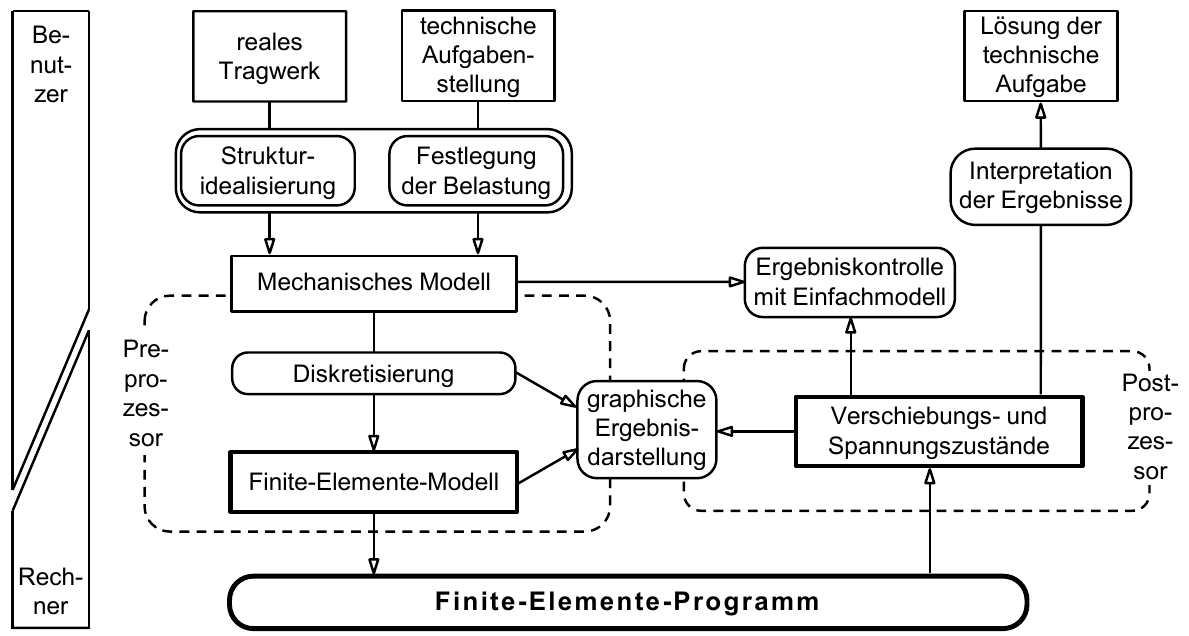
\includegraphics[width=0.7\linewidth]{files/Konstruktionsprozess-354f76ee1694c7cb48ad196b299f0eb9.png}
\caption[]{Einordnung numerischer Simulation in den Konstruktionsprozess nach \cite{knothe1991finite}}
\label{konstruktionsprozess}
\end{figure}

Finite-Elemente-Programme spielen eine wichtige Rolle bei der Untersuchung realer Tragwerke und technischer Aufgabenstellungen. Dieses leistungsfähige Tool ermöglicht es beispielsweise, die Integrität einer Pkw-Karosserie oder eines Rahmentragwerks zu analysieren, indem die Simulation eines Crash-Vorgangs durchgeführt wird oder die Traglast eines Bauteils berechnet wird. Für die virtuelle Produktentwicklung und eine prototypenfreie (oder prototypenarme) Entwicklung ist die Finite-Elemente-Methode aus den Entwicklungsabteilungen nicht mehr wegzudenken.

Der Weg zu einer validen FE-Simulation ist mehrstufig und interdisziplinär. In Abbildung Figure~\ref{konstruktionsprozess} sind die eigentlichen Schritte, die die Finite-Elemente-Methode betreffen, durch einen dicken Rahmen gekennzeichnet. Die vor- und nachgelagerte Prozesskette sollte von dem/der berechnenden Ingenieur/in eng begleitet werden, denn die Ergebnisse einer Simulation können nur so gut sein wie die Eingangsdaten: \textbf{Garbage in, garbage out}.

Zunächst wird die reale Struktur und ihre Belastung definiert und anschlie$\beta$end in geeigneter Weise abstrahiert:

\begin{itemize}
\item Genügt eine 2D-Berechnung oder gar eine 1D-Berechnung?
\item Welche geometrischen Details flie$\beta$en in die Simulation ein?
\item Kann ich die tatsächliche Last abstrahieren?
\item etc.
\end{itemize}

Das resultierende mechanische Modell ist somit eine idealisierte Darstellung der realen Problemstellung. Es geht darum, unwichtige Details wegzulassen, um die Berechnungen effizient und fokussiert zu halten, während gleichzeitig alle relevanten Belastungen präzise definiert werden müssen.

Auf die Modellierung folgt die Diskretisierung in finite Elemente. Dies sind kleine, standardisierte geometrische Objekte, auf denen die physikalischen Modellgleichungen gelöst werden. Mehr hierzu in späteren Kapiteln. Die Diskretisierung wird über sogenannte \textit{Preprozessoren} generiert. In modernen FE-Softwarepaketen sind diese Programmeinheiten integriert. Für gesonderte Diskretisierungsanforderungen gibt es jedoch auch Spezialsoftware wie:

\begin{itemize}
\item \href{https://altair.com/hypermesh/}{Hypermesh}
\item \href{https://www.beta-cae.com/}{Ansa}
\item \href{https://gmsh.info/}{Gmsh}
\end{itemize}

um nur einige zu nennen.
Zur Diskretisierung gehört nicht nur die Unterteilung des Gebietes in Finite Elemente. Auch die Belastungen müssen aus dem mechanischen Modell diskretisiert werden.

Das erstellte Finite-Elemente-Modell dient als Grundlage für die weiterführenden Berechnungen mit der gewählten FEM-Software - dem \textit{Prozessor}. Innerhalb des Programms wird aus den Eingabedaten ein, in der Regel nichtlineares, Gleichungssystem generiert und gelöst, das schlie$\beta$lich Aufschluss über relevante Grö$\beta$en wie Verschiebungen, Dehnungen, Spannungen, Wärmefluss und Temperaturverteilung gibt. Da die Menge an Ergebnisdaten bei gro$\beta$en Problemen erheblich sein kann, sind \textit{Postprozessoren} unverzichtbar, um eine übersichtliche und grafische Auswertung zu gewährleisten. Auch diese sind in kommerziellen FE-Systemen integriert, und auch hier haben sich für bestimmte Anwendungsfälle spezialisierte Softwarelösungen etabliert:

\begin{itemize}
\item \href{https://www.paraview.org/}{Paraview}
\item \href{https://tecplot.com/}{Tecplot}
\item \href{https://www.beta-cae.com/}{Ansa}
\item \href{https://www.gns-mbh.com/products/animator4/}{Animator4}
\end{itemize}

um auch hier nur einige zu nennen.

Der wichtigste Schritt für den/die Entwicklungsingenieur/in bei der FE-Simulation ist die anschlie$\beta$ende Auswertung und Bewertung der Ergebnisse. Man sollte den Resultaten stets mit einem gewissen Ma$\beta$ an Skepsis begegnen und entsprechende Kontrollen hinsichtlich Plausibilität und Grö$\beta$enordnung durchführen. Dies kann durch Vergleiche mit Einfachmodellen und experimentellen Untersuchungen unterstützt werden.

Letztlich muss der/die Anwender/in die Resultate im Kontext der technischen Aufgabe interpretieren. Sollten die Ergebnisse nicht zufriedenstellend sein, kann es notwendig sein, die Rechnung zu wiederholen. Dies kann Änderungen im Finite-Elemente-Modell, der Idealisierung der Struktur oder der Festlegung der Belastungen nach sich ziehen. Nur durch diese iterative Vorgehensweise lässt sich ein genaues und verlässliches Bild des untersuchten technischen Systems gewinnen.

%  -+-+-+-+-+-+-AI-SPLIT

%  - **Nutzung von Finite-Elemente-Programmen**
%   - Anwendung zur Untersuchung realer Tragwerke unter technischen Aufgabenstellungen
%   - Beispiele für reale Strukturen: Pkw-Karosserie, Stockwerkrahmen
%   - Beispiele für technische Aufgaben: Simulation eines Crash-Vorgangs, Ermittlung der Traglast
% 
% - **Erstellung des mechanischen Modells**
%   - Idealisierte Darstellung der Struktur entscheidend
%   - Weglassen von unwichtigen Strukturdetails
%   - Festlegung der relevanten Belastungen
% 
% - **Diskretisierung in finite Elemente**
%   - Manuelle Diskretisierung möglich bei kleinen Strukturen
%   - Rechnerunterstützung erforderlich bei komplexen Strukturen wie Fahrzeugkarosserien oder Flugzeugen
%   - Nutzung von Preprozessoren zur Modellerzeugung und grafischen Kontrolle
% 
% - **Finite-Elemente-Modell als Basis für Berechnungen**
%   - Bereitstellung von Eingabedaten für FEM-Programme
%   - Internes Generieren und Lösen von Gleichungssystemen
%   - Bestimmung relevanter Größen wie Verschiebungen und Schnittkräfte
%   - Verwendung von Postprozessoren zur übersichtlichen Darstellung der Ergebnisse
% 
% - **Kritische Bewertung der FEM-Ergebnisse**
%   - Notwendigkeit des Misstrauens gegenüber FEM-Ergebnissen
%   - Durchführung von Kontrollen für Plausibilität und Größenordnung der Ergebnisse
%   - Vergleich mit Einfachmodellen und experimentellen Untersuchungen
% 
% - **Interpretation und Anpassung**
%   - Interpretation der Ergebnisse im Kontext der technischen Aufgabe
%   - Mögliche Wiederholung der Rechnung bei nicht zufriedenstellenden Ergebnissen
%   - Anpassung des Finite-Elemente-Modells, Idealisierung der Struktur oder Belastungsfestlegung ggf. notwendig

\subsubsection{Der Systembegriff}

\begin{quote}
Ein System besteht aus einer Menge von Elementen (Teilsystemen), die Eigenschaften besitzen und durch Beziehungen miteinander verknüpft sind. Das System wird durch eine Systemgrenze von der Umgebung abgegrenzt und steht mit der Umgebung durch Ein- und Ausgangsgrö$\beta$en in Beziehung. Die Funktion eines Systems kann durch den Unterschied der dem Zweck entsprechenden Ein- und Ausgangsgrö$\beta$en beschrieben werden. Die Systemelemente können selbst wiederum Systeme sein, die aus Elementen und Beziehungen bestehen. \cite{ehrlenspiel2013integrierte}
\end{quote}

Die Definition eines Systems umfasst mehrere wesentliche Schritte:

\begin{enumerate}
\item \textbf{Identifikation der Systemgrenzen}: Hier wird festgelegt, was zum System gehört und was nicht. Diese Abgrenzung ist entscheidend, um den Fokus der Analyse zu bestimmen und irrelevante Einflüsse auszuschlie$\beta$en.


\item \textbf{Bestimmung der Systemelemente}: In diesem Schritt werden die Komponenten identifiziert, die Teil des Systems sind. Diese Komponenten können physikalische Objekte, biologische Organismen, soziale Gruppen, technische Bauteile etc. sein.


\item \textbf{Beschreibung der Beziehungen zwischen den Systemelementen}: Hier wird untersucht, wie die einzelnen Komponenten miteinander interagieren.
\end{enumerate}

Ein gut definiertes System ist entscheidend für die Genauigkeit und Zuverlässigkeit der Simulationsergebnisse. Nur wenn alle relevanten Komponenten und deren Interaktionen korrekt erfasst und modelliert werden, können valide Aussagen über das Systemverhalten getroffen werden.

\textbf{Zustand, Zustandsgrö$\beta$e, Zustandsvariable}

In der numerischen Simulation wird der Zustand eines Systems durch eine Reihe von Zustandsgrö$\beta$en oder Zustandsvariablen beschrieben. Diese Variablen repräsentieren die Eigenschaften des Systems zu einem bestimmten Zeitpunkt.

\begin{itemize}
\item \textbf{Zustand}: Der Zustand eines Systems ist eine vollständige Beschreibung des Systems zu einem bestimmten Zeitpunkt. Er umfasst alle relevanten Informationen, die notwendig sind, um das Verhalten des Systems zu verstehen und vorherzusagen. Der Zustand ist somit eine Momentaufnahme des Systems, die alle wesentlichen Eigenschaften und Charakteristika beinhaltet.


\item \textbf{Zustandsgrö$\beta$e / Zustandsvariable}: Eine Zustandsgrö$\beta$e ist eine messbare Eigenschaft des Systems, die den Zustand des Systems beschreibt. Beispiele für Zustandsgrö$\beta$en sind Temperatur, Druck, Spannung und Verformung. Diese Grö$\beta$en sind oft physikalische Messwerte, die direkt beobachtet oder gemessen werden können. Es handelt sich bei Zustandsvariablen zudem meist um Felder, das hei$\beta$t, sie haben eine räumliche und zeitliche Abhängigkeit.


\item \textbf{Systemverhalten}: Das Systemverhalten beschreibt, wie sich das System im Laufe der Zeit entwickelt. Es umfasst die Dynamik und die Reaktionen des Systems auf äu$\beta$ere Einflüsse und interne Prozesse. Das Systemverhalten ist somit die zeitliche Entwicklung des Zustands des Systems und kann durch die zeitliche Abfolge von Punkten im Zustandsraum beschrieben werden.
\end{itemize}

%  -+-+-+-+-+-+-AI-SPLIT

\subsubsection{Klassifikation von Systemen}

Systeme können nach verschiedenen Ordnungskriterien klassifiziert werden. In der nachfolgenden Tabelle sind die wichtigsten Kriterien und deren Beschreibung aufgeführt.

\bigskip\noindent
\begin{tabular}{p{\dimexpr 0.500\linewidth-2\tabcolsep}p{\dimexpr 0.500\linewidth-2\tabcolsep}}
\toprule
\textbf{Klassifikation} & \textbf{Beschreibung} \\
\hline
\textbf{Statisch} & Systeme, deren Verhalten unabhängig von der Zeit ist; Zustände ändern sich nicht. \\
\textbf{Quasistatisch} & Systeme, die sich langsam ändern, sodass sie zu jedem Zeitpunkt als statisch betrachtet werden können. \\
\textbf{Dynamisch} & Systeme, deren Verhalten sich mit der Zeit ändert; Zustände entwickeln sich über die Zeit. \\
\textbf{Zeitkontinuierlich} & Systeme, die zu jedem Zeitpunkt einen definierten Zustand haben; Änderungen erfolgen kontinuierlich. \\
\textbf{Zeitdiskret} & Systeme, die nur zu bestimmten Zeitpunkten Zustandsänderungen aufweisen; Änderungen erfolgen in diskreten Schritten. \\
\textbf{Ereignisorientiert} & Systeme, deren Verhalten durch bestimmte Ereignisse ausgelöst wird; Änderungen treten in Reaktion auf Ereignisse auf. \\
\textbf{Deterministisch} & Systeme, deren Verhalten vollständig durch Anfangsbedingungen und Regeln bestimmt ist; keine Zufälligkeit. \\
\textbf{Stochastisch} & Systeme, deren Verhalten durch Zufallsprozesse beeinflusst wird; es gibt eine gewisse Unsicherheit im Verhalten. \\
\bottomrule
\end{tabular}

\bigskip\begin{figure}[!htbp]
\centering
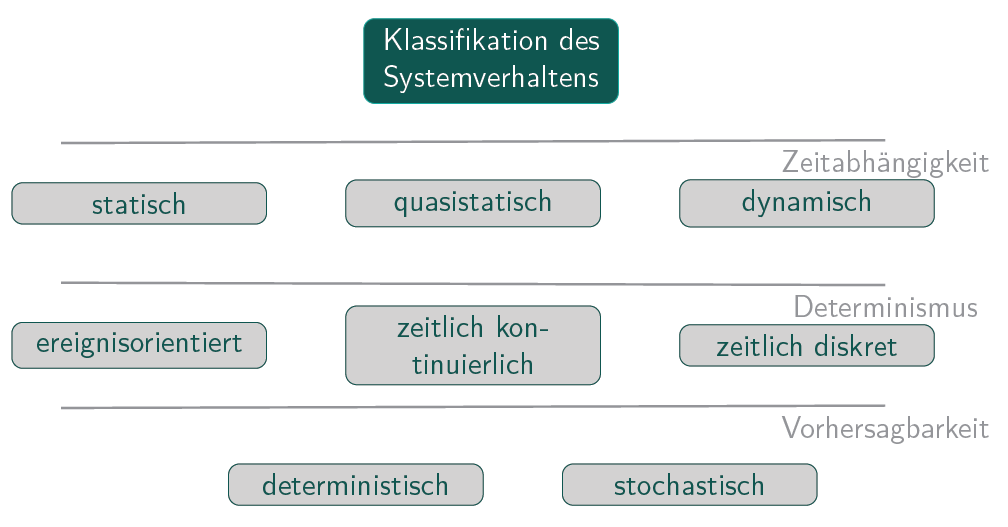
\includegraphics[width=0.7\linewidth]{files/Systemverhalten-eb19fad1d9ad10e9c65047ac7b46ad78.png}
\caption[]{Klassifikation von Systemen nach ihrem Verhalten}
\label{systemverhalten}
\end{figure}

\subsubsection{Der Modellbegriff}

In der Entwicklung mechatronischer Systeme spielen die VDI-Richtlinien 2206 und 2211 eine zentrale Rolle. Diese Richtlinien bieten eine methodische Grundlage für die Modellbildung, die ein physikalisch-mathematisches Abbild eines technischen Bauelements, einer Baugruppe oder eines komplexen Systems darstellt.

\textbf{Modellbildung und ihre Bedeutung}

Modelle sind materielle oder immaterielle Gebilde, die geschaffen werden, um für einen bestimmten Zweck ein Original zu repräsentieren. Sie können als Abbildungen oder Nachbildungen von Originalen betrachtet werden. Die Modellbildung beinhaltet die Darstellung eines physikalisch-mathematischen Modells eines vorhandenen Systems oder eines zu entwickelnden Systems. Der Zweck der Modellbildung besteht darin, das Original durch das Modell zu ersetzen und es als Stellvertreter des Originals zu nutzen, um Rückschlüsse auf das Original zu ziehen.

Modelle können somit als zweckgerichtete, vereinfachte Abbildungen oder Nachbildungen von Originalen aufgefasst werden. Sie umfassen eine Vielzahl von Konstrukten, darunter Anschauungsmodelle, Prototypen, Konstruktionszeichnungen, Schaltpläne, mathematische Gleichungen, aber auch Gedankenmodelle bzw. mentale Modelle, Vorstellungen und Bilder.

\textbf{Anforderungen an Modelle}

Modelle müssen original- und realitätsnah sein, um charakteristische Eigenschaften und Verhalten des Originals genau zu beschreiben. Der Modellzweck hängt von den Lebensphasen des Produkts ab, und es ist wichtig, ein angemessenes Aufwand-/Nutzen-Verhältnis zu gewährleisten. Der Aufwand für Modellierung und Analyse ist eng mit dem Detaillierungsgrad (Granularität) des Modells verbunden. Eine sehr genaue Modellierung ist nicht immer notwendig; Unsicherheiten können den Nutzen eines detaillierten Modells in Frage stellen.

Das Modellverhalten muss im Gültigkeitsbereich dem realen Systemverhalten entsprechen, um die Modellgültigkeit zu gewährleisten. Das Verhalten resultiert aus den Eigenschaften der Modellelemente und deren Verknüpfungen. Bei mehreren geeigneten Modellierungsansätzen sollte die einfachste Methode bevorzugt werden, um die Modelleffizienz zu maximieren. Es gibt keine allgemeinen Regeln für die Herleitung eines einfachen, effizienten und gültigen Modells; vielmehr sind Erfahrung und Vorwissen entscheidend.

%  -+-+-+-+-+-+-AI-SPLIT

\subsubsection{Modellbildung}

\begin{framed}
\textbf{Ziel der Modellbildung}\\
Modellbildung ist die Schaffung eines Modells, das dem Untersuchungszweck entspricht und demgemä$\beta$ verändert und ausgewertet werden kann, um damit Rückschlüsse auf das Original ziehen zu können.
\end{framed}

\begin{figure}[!htbp]
\centering
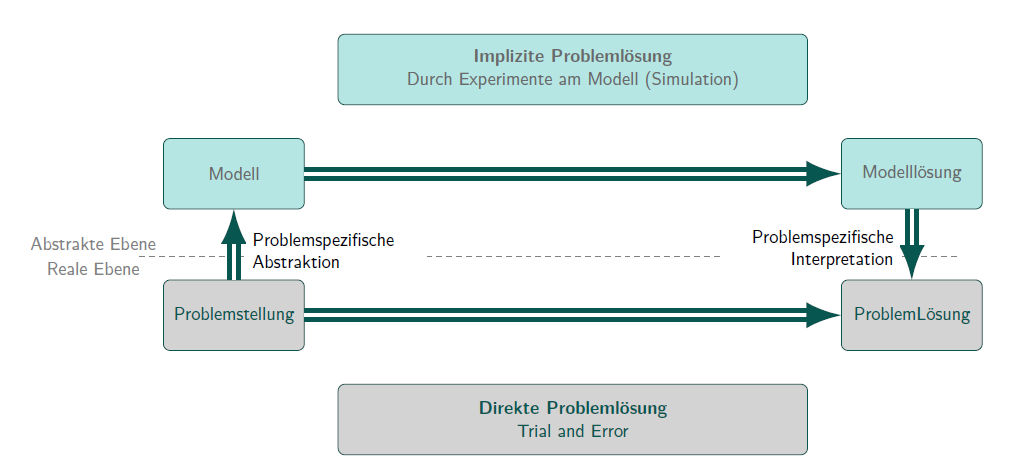
\includegraphics[width=0.7\linewidth]{files/Problemloesung-e104c317db14666b2fd6f513a8ca1a48.png}
\caption[]{Problemlösung im Ingenieurwesen nach \cite{vajna2009cax}}
\label{problemlösung}
\end{figure}

Die Modellabstraktion ist ein zentraler Bestandteil der Ingenieurwissenschaft, da sie die Realität einer Berechnung zugänglich macht. Durch die Abstraktion werden irrelevante Details vernachlässigt, während die relevanten Details erhalten bleiben. Das Ziel ist es, ein Modellergebnis zu erzielen, das eine hohe Relevanz für die Lösung der realen Problemstellung aufweist.

\textbf{Modellabstraktion als Grundlage für Analyse und Design}

Ein Modell dient als Grundlage für die Analyse und das Design von Systemen. Durch die Konzentration auf die spezifischsten und wichtigsten Merkmale und die Abstraktion von unwichtigen Eigenschaften und Details wird die Komplexität der Problemstellung reduziert. Diese Vereinfachung ist bereits ein Ziel der Analyse, da sie die Handhabbarkeit der Problemstellung ermöglicht. Ohne eine solche Vereinfachung wären viele Problemstellungen innerhalb der praktischen Beschränkungen von Zeit und Ressourcen äu$\beta$erst komplex zu simulieren oder nicht effektiv zu analysieren.

\textbf{Vorteile einfacher Modelle}

Einfachere Modelle sind von Natur aus leichter zu entwickeln, zu verstehen und zu modifizieren. Dies ist besonders wertvoll in iterativen Designprozessen, in denen häufige Aktualisierungen von Modellen erforderlich sind. Abstrakte Modelle können als gemeinsame Sprache für Ingenieure aus verschiedenen Disziplinen oder mit unterschiedlichem Fachwissen dienen. Sie reduzieren Missverständnisse und ermöglichen eine effektivere Zusammenarbeit in Ingenieurprojekten.

Darüber hinaus erfordern einfachere Modelle weniger Rechenleistung und Zeit für die Lösung. Dies ermöglicht mehr Iterationen, Sensitivitätsanalysen und die Untersuchung von Designalternativen innerhalb angemessener Zeitrahmen. Die Vereinfachung durch Modellabstraktion trägt somit wesentlich zur Effizienz und Effektivität des gesamten Design- und Analyseprozesses bei.

\begin{figure}[!htbp]
\centering
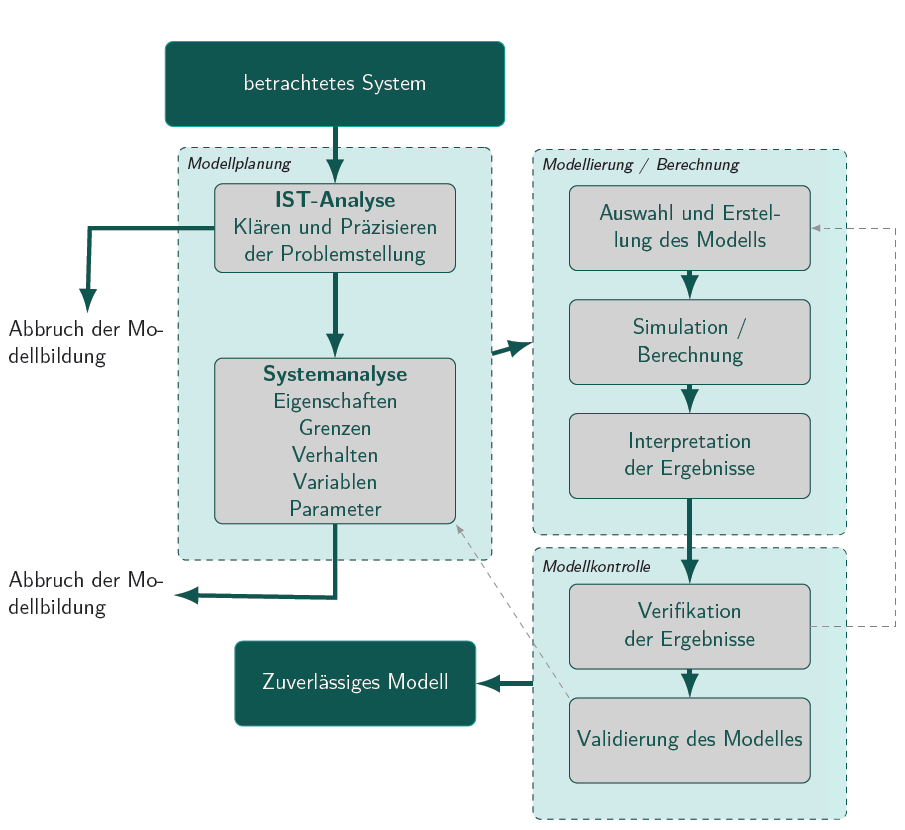
\includegraphics[width=0.7\linewidth]{files/Modellbildung-df30eb7519c2d11046de71abe95091b6.png}
\caption[]{Modellbildungsprozess nach \cite{vajna2009cax}}
\label{modellbildung}
\end{figure}

In Abbildung Modellbildung ist der Modellbildungsprozess dargestellt. Die Modellplanung beginnt mit einer IST-Analyse, in der die Aufgabenstellung zu klären und zu präzisieren ist. Dabei treten typischerweise Fragen auf wie (\cite{vajna2009cax}):

\begin{itemize}
\item Was ist das zu untersuchende Original (System, Elemente, Systemgrenzen)?
\item Welche Fragestellungen sollen behandelt werden (Festlegung des Modellzwecks)?
\item Welche Sichtweisen auf das zu untersuchende Original (Systemaspekte, Bewertungskriterien) sind für den Modellzweck notwendig?
\item Welche Eigenschaften müssen für die gewünschte Bewertung (z.~B. zur Eigenschaftsabsicherung) herangezogen werden?
\item Welche Effekte (Details) müssen daher berücksichtigt oder können vernachlässigt werden?
\item Welche Testsituationen sind zu untersuchen („Lastfälle``, Testszenarien, „Use Cases``)?
\item Welche Parameter bzw. Zustandsgrö$\beta$en eines mathematischen Modells werden als vorgegeben (Parameter), welche als Zustandsvariablen betrachtet?
\item Welche Ergebnisse sind zur Klärung der Fragestellungen erforderlich und in welcher Form sollen die Ergebnisdaten aufbereitet und dokumentiert werden (Ergebnisdarstellung und Dokumentation)?
\item Welche Relevanz und Signifikanz haben die zu erwartenden Ergebnisse in Bezug auf die Fragestellungen? Wird die Fragestellung durch die Ergebnisse auch wirklich beantwortet?
\end{itemize}

%  -+-+-+-+-+-+-AI-SPLIT

\textbf{Verifikation und Validierung}

Jedes Modell stellt lediglich eine mehr oder weniger genaue Annäherung an das Original (z.B. ein reales System) dar. Daher ist es nach der Modellentwicklung notwendig, zu überprüfen, ob das Modell mit seinen Idealisierungen das zu untersuchende Original ausreichend genau abbildet. Die Verifikation untersucht, ob sich das Modell grundsätzlich plausibel verhält, und bezieht sich dabei auf das Modellverhalten, unabhängig von Vergleichen mit einem konkreten Original. Die Modellverifikation betrifft somit die Überprüfung der Plausibilität des Modellverhaltens an sich, also für „fiktive`` Originale. Die Validierung hingegen liefert eine Aussage darüber, ob das erstellte Modell konkrete Originale hinreichend beschreibt und in welchem Bereich das Modell gültig ist (Grenzen des Modells).

\subsubsection{Ansätze zur Abstraktion mechanischer Modelle}

Zur Abstraktion mechanischer Modelle können folgende Ansätze angewendet werden:

\begin{enumerate}
\item Vereinfachung der Geometrie

\begin{itemize}
\item Abstraktion durch einfachere geometrische Grundkörper
\item Komplexe Maschinenrahmen als Skelettstruktur aus Balken oder ein dünnwandiges Druckgefä$\beta$ als Schale modelliert werden
\end{itemize}


\item Dimensionsreduktion

\begin{itemize}
\item Übergang von einer 3D-Darstellung zu einer 2D-Darstellung (ebener Spannungszustand, ebener Dehnungszustand, rotationssymmetrisch) oder sogar 1D-Darstellung (Balken, Stäbe)
\end{itemize}


\item Vereinfachung der Materialeigenschaften

\begin{itemize}
\item Wenn angemessen, linear-elastische Materialmodelle anstelle komplexerer nichtlinearer oder anisotroper Modelle
\end{itemize}


\item Abstraktion der Randbedingungen

\begin{itemize}
\item Darstellung komplexer Lagerungen oder Lasten durch idealisierte Randbedingungen
\item Z. B. feste, gelenkige oder rollende Lagerungen oder durch die Verwendung von Punktlasten oder verteilten Lasten
\end{itemize}


\item Systemebenenabstraktion

\begin{itemize}
\item Subsysteme oder Komponenten werden als Black Boxes mit definierten Ein- und Ausgängen modelliert
\item Schwerpunkt auf ihrem Gesamtverhalten und nicht auf komplizierten internen Details
\item Ansatz besonders nützlich für die Analyse gro$\beta$er, komplexer Systeme, indem diese in kleinere, besser handhabbare Teile zerlegt werden
\end{itemize}


\item Vereinfachte physikalische Bilanzgleichung
\end{enumerate}

%  -+-+-+-+-+-+-AI-SPLIT

\begin{framed}
\textbf{Fragen zum Kapitel}\\
\textbf{Allgemeine Verständnisfragen zur numerischen Simulation}

\begin{itemize}
\item Was sind mögliche Zielstellungen der numerischen Simulation im Konstruktionsprozess?
\item Erläutern Sie den Begriff ``Garbage in, garbage out'' im Kontext von Finite-Elemente-Simulationen.
\item Beschreiben Sie die Schritte, die vor einer FE-Simulation durchgeführt werden müssen.
\item Nennen Sie zwei Kriterien für die Wahl zwischen einer 1D-, 2D- oder 3D-Finite-Elemente-Berechnung.
\end{itemize}

\textbf{Zum Thema Systembegriff}

\begin{itemize}
\item Wie wird ein System definiert und welche Elemente umfasst es?
\item Was sind die wesentlichen Schritte bei der Definition eines Systems?
\item Was versteht man unter Zustand und Zustandsgrö$\beta$e in der numerischen Simulation?
\end{itemize}

\textbf{Zur Klassifikation von Systemen}

\begin{itemize}
\item Nennen Sie drei Kriterien zur Klassifikation von Systemverhalten und beschreiben Sie diese.
\item Warum ist das Wissen über das Systemverhalten wichtig für die Simulation?
\end{itemize}

\textbf{Über den Modellbegriff}

\begin{itemize}
\item Welche Anforderungen sollten Modelle erfüllen?
\item Erklären Sie den Begriff ``Modellabstraktion'' und dessen Bedeutung im Ingenieurwesen.
\item Welche Vorteile bieten einfachere Modelle gegenüber komplexeren Modellen während des Design- und Analyseprozesses?
\end{itemize}

\textbf{Zum Modellbildungsprozess}

\begin{itemize}
\item Nennen Sie die wesentlichen Schritte im Modellbildungsprozess.
\item Welche Bedeutung haben Verifikation und Validierung in der Modellbildung?
\end{itemize}

\textbf{Ansätze zur Abstraktion mechanischer Modelle}

\begin{itemize}
\item Nennen Sie drei Ansätze zur Abstraktion mechanischer Modelle und erklären Sie diese kurz.
\item Was versteht man unter Dimensionsreduktion und wann wird sie angewendet?
\item In welchen Situationen ist eine Vereinfachung der Materialeigenschaften angebracht?
\end{itemize}

\textbf{Vertiefende Fragen zur Reflexion}

\begin{itemize}
\item Was ist der Unterschied zwischen der Verifikation und der Validierung eines Modells?
\item Was sind die Konsequenzen einer unzureichenden Modellvalidierung?
\item Wie kann eine kritische Bewertung der Ergebnisse einer FE-Simulation erfolgen?
\end{itemize}
\end{framed}